\documentclass[aspectratio=169,10pt]{beamer}

\usepackage[T1]{fontenc}
\usepackage{lmodern}
\usepackage{graphicx}
\usepackage{booktabs}
\usepackage{tikz}
\usetikzlibrary{arrows.meta,calc,positioning,shapes.geometric}

\definecolor{Ink}{HTML}{12202B}
\definecolor{Muted}{HTML}{586875}
\definecolor{Paper}{HTML}{F5F7F8}
\definecolor{Rule}{HTML}{D9E0E4}
\definecolor{Blue}{HTML}{1261A0}
\definecolor{BlueLight}{HTML}{E8F2FA}
\definecolor{Cyan}{HTML}{16A6B6}
\definecolor{CyanLight}{HTML}{E4F7F8}
\definecolor{Orange}{HTML}{E97824}
\definecolor{OrangeLight}{HTML}{FFF0E5}
\definecolor{Green}{HTML}{248A62}
\definecolor{GreenLight}{HTML}{E7F5EF}
\definecolor{Red}{HTML}{B84A4A}

\setbeamercolor{normal text}{fg=Ink,bg=white}
\setbeamercolor{frametitle}{fg=Ink,bg=white}
\setbeamerfont{frametitle}{size=\Large,series=\bfseries}
\setbeamertemplate{navigation symbols}{}
\setbeamertemplate{frametitle}{%
  \vspace{0.20cm}\insertframetitle\par%
  \vspace{-0.05cm}\color{Rule}\rule{\textwidth}{0.6pt}}
\setbeamersize{text margin left=0.62cm,text margin right=0.62cm}

\newcommand{\sectionlabel}[1]{\textcolor{Muted}{\scriptsize\bfseries\MakeUppercase{#1}}}
\newcommand{\metric}[3]{%
  \begin{tikzpicture}[baseline=(value.base)]
    \node[rounded corners=2pt,fill=#1,inner xsep=5pt,inner ysep=3pt] (value)
      {\textcolor{white}{\bfseries #2}\;\textcolor{white}{\scriptsize #3}};
  \end{tikzpicture}}

\begin{document}

% Slide 1 --------------------------------------------------------------------
\begin{frame}[t]{VisACD $\longrightarrow$ visacd\_batched}
  \vspace{-0.10cm}
  {\small\textcolor{Muted}{Same visibility-based decomposition; a new single-GPU throughput engine.}}

  \vspace{0.10cm}
  \begin{center}
    \includegraphics[trim=0 475 0 475,clip,width=0.92\textwidth]{visuals/teaser.png}
  \end{center}
  \vspace{-0.15cm}

  \begin{columns}[T,totalwidth=\textwidth]
    \begin{column}{0.335\textwidth}
      \sectionlabel{Baseline VisACD}
      \vspace{0.07cm}

      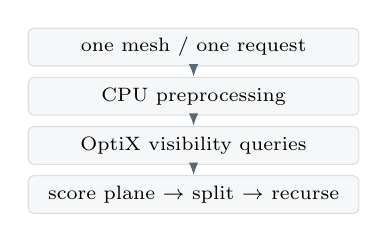
\begin{tikzpicture}[
          node distance=0.13cm,
          stage/.style={draw=Rule,fill=Paper,rounded corners=2pt,
            minimum width=4.20cm,minimum height=0.48cm,font=\scriptsize,align=center},
          flow/.style={-{Latex[length=1.6mm]},draw=Muted,line width=0.55pt}]
        \node[stage] (in) {one mesh / one request};
        \node[stage,below=of in] (pre) {CPU preprocessing};
        \node[stage,below=of pre] (optix) {OptiX visibility queries};
        \node[stage,below=of optix] (split) {score plane $\rightarrow$ split $\rightarrow$ recurse};
        \draw[flow] (in)--(pre);
        \draw[flow] (pre)--(optix);
        \draw[flow] (optix)--(split);
      \end{tikzpicture}

      \vspace{0.11cm}
      \begin{beamercolorbox}[wd=\linewidth,sep=0.10cm,rounded=true]{normal text}
        \color{Red}\scriptsize\bfseries Throughput limit\par
        \color{Muted}\scriptsize Phase barriers, repeated setup and host--device traffic leave gaps between irregular jobs.
      \end{beamercolorbox}
    \end{column}

    \begin{column}{0.055\textwidth}
      \vspace{1.33cm}
      \centering
      
\begin{tikzpicture}
        \draw[-{Latex[length=2.4mm]},line width=1.2pt,Blue] (0,0)--(0.55,0);
      \end{tikzpicture}
    \end{column}

    \begin{column}{0.61\textwidth}
      \sectionlabel{Batched execution engine}
      \vspace{0.07cm}

      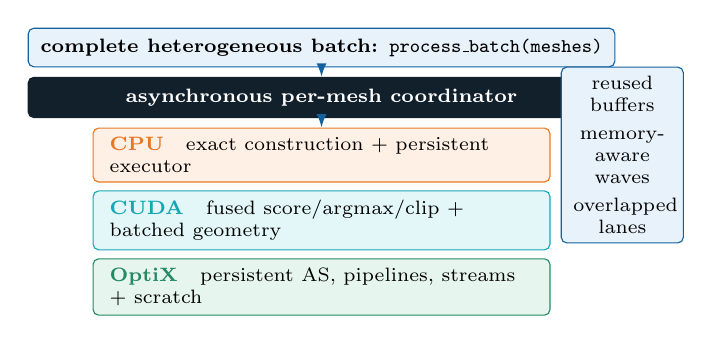
\begin{tikzpicture}[
          lane/.style={rounded corners=2pt,minimum height=0.56cm,font=\scriptsize,
            align=left,text width=5.38cm,inner xsep=6pt},
          flow/.style={-{Latex[length=1.7mm]},draw=Blue,line width=0.65pt}]
        \node[draw=Blue,fill=BlueLight,rounded corners=2pt,minimum width=7.45cm,
          minimum height=0.49cm,font=\scriptsize\bfseries] (batch)
          {complete heterogeneous batch: \texttt{process\_batch(meshes)}};
        \node[draw=Ink,fill=Ink,text=white,rounded corners=2pt,below=0.12cm of batch,
          minimum width=7.45cm,minimum height=0.51cm,font=\scriptsize\bfseries] (coord)
          {asynchronous per-mesh coordinator};
        \node[lane,draw=Orange,fill=OrangeLight,below=0.12cm of coord]
          (cpu) {\textcolor{Orange}{\bfseries CPU}\quad exact construction + persistent executor};
        \node[lane,draw=Cyan,fill=CyanLight,below=0.10cm of cpu] (cuda)
          {\textcolor{Cyan}{\bfseries CUDA}\quad fused score/argmax/clip + batched geometry};
        \node[lane,draw=Green,fill=GreenLight,below=0.10cm of cuda] (optix)
          {\textcolor{Green}{\bfseries OptiX}\quad persistent AS, pipelines, streams + scratch};
        \node[draw=Blue,fill=BlueLight,rounded corners=2pt,right=0.13cm of cpu,
          minimum width=1.55cm,minimum height=1.85cm,text width=1.24cm,
          align=center,font=\scriptsize] (reuse) {reused buffers\\[2pt]memory-aware waves\\[2pt]overlapped lanes};
        \coordinate (join) at ($(cuda.east)!0.5!(reuse.west)$);
        \draw[flow] (batch)--(coord);
        \draw[flow] (coord.south) -- ++(0,-0.07) -| (cpu.north);
      \end{tikzpicture}
    \end{column}
  \end{columns}

  \vspace{0.05cm}
  \begin{beamercolorbox}[wd=\dimexpr\textwidth-0.24cm\relax,sep=0.12cm,rounded=true]{normal text}
    \color{Ink}\small\bfseries Same visibility objective and quality controls. \textcolor{Blue}{Deterministic batches keep the GPU fed.}
  \end{beamercolorbox}
\end{frame}

% Slide 2 --------------------------------------------------------------------
\begin{frame}[t]{Three 200-mesh workloads: $12.9$--$25.5\times$ faster}
  \vspace{-0.12cm}
  \begin{columns}[T,totalwidth=\textwidth]
    \begin{column}{0.555\textwidth}
      \sectionlabel{End-to-end speedup vs. original \texttt{process} $\times 200$}
      \vspace{0.06cm}

      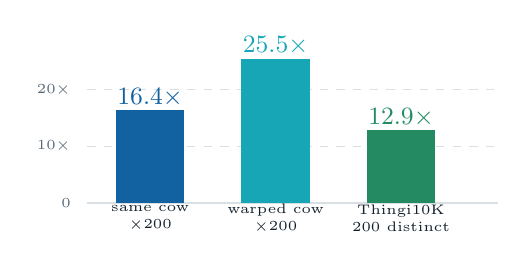
\begin{tikzpicture}[x=0.88cm,y=0.72cm]
        \draw[Rule,line width=0.55pt] (0.62,0.18)--(6.55,0.18);
        \foreach \y/\lab in {1.0/10,2.0/20} {
          \draw[Rule,dashed] (0.62,\y+0.18)--(6.55,\y+0.18);
          \node[font=\tiny,text=Muted,anchor=east] at (0.52,\y+0.18) {\lab$\times$};
        }
        \node[font=\tiny,text=Muted,anchor=east] at (0.52,0.18) {0};
        \fill[Blue] (1.03,0.18) rectangle (2.02,1.821);
        \fill[Cyan] (2.84,0.18) rectangle (3.83,2.728);
        \fill[Green] (4.65,0.18) rectangle (5.64,1.469);
        \node[font=\small\bfseries,text=Blue] at (1.525,2.04) {$16.4\times$};
        \node[font=\small\bfseries,text=Cyan] at (3.335,2.95) {$25.5\times$};
        \node[font=\small\bfseries,text=Green] at (5.145,1.69) {$12.9\times$};
        \node[font=\tiny,text=Ink,align=center] at (1.525,-0.09) {same cow\\$\times 200$};
        \node[font=\tiny,text=Ink,align=center] at (3.335,-0.09) {warped cow\\$\times 200$};
        \node[font=\tiny,text=Ink,align=center] at (5.145,-0.09) {Thingi10K\\200 distinct};
      \end{tikzpicture}

      \vspace{0.00cm}
      {\tiny
      \renewcommand{\arraystretch}{1.03}
      \begin{tabular}{@{}l r r r@{}}
        \toprule
        \textbf{input set} & \textbf{original} & \textbf{batched} & \textbf{speedup} \\
        \midrule
        identical cow & 57.8767 s & 3.5276 s & $16.4\times$ \\
        smooth variants & 90.5219 s & 3.5522 s & $25.5\times$ \\
        Thingi10K & 130.3480 s & 10.1113 s & $12.9\times$ \\
        \bottomrule
      \end{tabular}}

      \vspace{0.08cm}
      \begin{beamercolorbox}[wd=\dimexpr\linewidth-0.12cm\relax,sep=0.06cm,rounded=true]{normal text}
        \tiny\textcolor{Blue}{\bfseries Diversity ladder}\quad
        1 geometry hash $\rightarrow$ 200 smooth unique hashes (1.02\% median RMS warp)
        $\rightarrow$ 11 categories, 116--48,023 vertices
      \end{beamercolorbox}
    \end{column}

    \begin{column}{0.415\textwidth}
      \sectionlabel{What moved the needle}
      \vspace{0.08cm}

      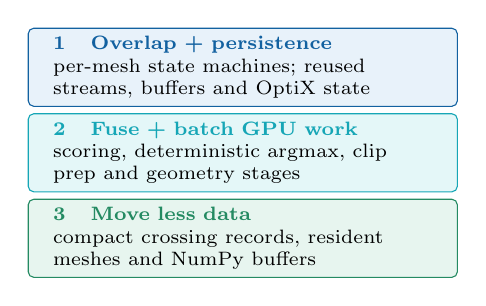
\begin{tikzpicture}[
          lever/.style={rounded corners=2pt,minimum width=5.45cm,text width=4.82cm,
            align=left,inner xsep=8pt,inner ysep=3pt,font=\scriptsize}]
        \node[lever,draw=Blue,fill=BlueLight] (one)
          {\textcolor{Blue}{\bfseries 1\quad Overlap + persistence}\par
           per-mesh state machines; reused streams, buffers and OptiX state};
        \node[lever,draw=Cyan,fill=CyanLight,below=0.08cm of one] (two)
          {\textcolor{Cyan}{\bfseries 2\quad Fuse + batch GPU work}\par
           scoring, deterministic argmax, clip prep and geometry stages};
        \node[lever,draw=Green,fill=GreenLight,below=0.08cm of two] (three)
          {\textcolor{Green}{\bfseries 3\quad Move less data}\par
           compact crossing records, resident meshes and NumPy buffers};
      \end{tikzpicture}

      \vspace{0.03cm}
      \metric{Orange}{+24.7\%}{surface preprocessing @ $n=200$}

      \vspace{0.03cm}
      \metric{Green}{91\%}{less clip D$\rightarrow$H traffic}

      \vspace{0.03cm}
      {\tiny\textcolor{Muted}{Dense-resident exact preprocessing on Thingi10K: 10.2873 s $\rightarrow$ \textbf{10.0478 s} ($+2.3\%$; 7-run medians), same digest. The timing ranges overlap, so it remains opt-in.}}
    \end{column}
  \end{columns}

  \vspace{0.01cm}
  {\fontsize{4.6}{5.2}\selectfont
    \textcolor{Green}{\bfseries Exactness:} 33/33 surface + 44/44 full-remesh cases; scheduling matrices matched; Compute Sanitizer: 0 errors/hazards.}

  \vspace{0.02cm}
  {\fontsize{4.0}{4.6}\selectfont\textcolor{Muted}{Medians of 3; concavity 0.04; 2 parts; conversion excluded. RTX 5090, CUDA 12.8, Threadripper PRO 9955WX. Original \texttt{3d9327b}; current \texttt{01e398c}; Thingi10K manifest \texttt{efbf9ed9b385cf9f}. Pills: replicated-cow diagnostics.}}
\end{frame}

\end{document}
